% Time-stamp: Mon Jun 24 18:01:48 2013
\chapter{Vectors and Motion along Space Curves}

\section{Vectors} %{{{1

\subsection{Geometric description of vectors} %{{{2
\label{sec:geometric-description-of-vectors}
A vector is an arrow connecting two points.  If the points are $A$ and
$B$ then we call the vector $\tpv AB$. If we translate a vector $\tpv
AB$ \emph{without turning it} then we say that the resulting vector
$\tpv CD$ is the same vector as the original vector $\tpv AB$.  We say
that the arrows $\tpv AB$ and $\tpv PQ$ \emph{both represent the same
  vector.}
\begin{figure}[h]\centering
  \input ../figures/234/005equalvectors.tex
  \caption{$\tpv AB$ and $\tpv CD$ represent the same vector}
\end{figure}
Since both $\tpv AB$ and $\tpv PQ$ are the same vector we will often
want to use a notation for vectors that does not emphasize any
particular choice of initial-~and endpoint.  The notation we will use
in this course is
\[
\va = \tpv AB = \tpv PQ,
\]
i.e., a single letter with an arrow on top will always stand for a
vector in this course.

\begin{figure}[h]\centering
  \def\figfont{\sffamily\footnotesize\color{darkbluegreen}\centering}
  \def\addingvectorsCapA{\parbox{1in}{\figfont%
      to add\\
      two vectors\dots}} \def\addingvectorsCapB{\parbox{1in}{\figfont%
      \dots move one vector until its initial point\dots}}
  \def\addingvectorsCapC{\parbox{1in}{\figfont%
      \dots is the end point of the other\dots} }
  \def\addingvectorsCapD{\parbox{1in}{\figfont%
      \dots and combine them.} } \input
  ../figures/234/005adding-vectors2.pdf_tex
  \caption{Adding vectors}
\end{figure}
\subsection{Arithmetic of vectors} %{{{2
\label{sec:arithmetic-of-vectors}
To add two vectors $\tpv AB$ and $\tpv PQ$ we first translate the vector $\tpv PQ$ so
that its initial point becomes $B$; let the result of this translation be the vector
$\tpv BC$.  Then the sum of $\tpv AB$ and $\tpv PQ$ is $\tpv AC$: in a formula,
\[
\tpv AB + \tpv PQ = \tpv AB + \tpv BC = \tpv AC.
\]
A different way of adding two vectors $\tpv AB$ and $\tpv PQ$ is to move the vectors
around until they have the same initial point.  Two vectors with a common initial
point form two sides of a parallelogram (see
Figure~\ref{fig:adding-vectors-parallelogram}) and the sum of the two vectors is the
diagonal of that parallelogram.
\begin{figure}[h]
  \input ../figures/234/005adding-vectors-parallelogram.pdf_tex
  \caption{{\bfseries Using a parallelogram to add vectors. }
  To find $\tpv AB  + \tpv AD$ we move the vector $\tpv AD$ so that its initial point
  is at $B$, i.e.~the endpoint of $\tpv AB$.  This gives us a 
  parallelogram $ABCD$, where $\tpv AD = \tpv BC$.  Therefore $\tpv AB+\tpv AD = \tpv
  AB+\tpv BC = \tpv AC$ }
  \label{fig:adding-vectors-parallelogram}
\end{figure}

One can also multiply vectors with numbers.  To multiply a vector $\va$ with a
positive real number $t>0$, we multiply the length of the vector by a factor $t$,
without changing the direction of the vector.
\begin{figure}[h]
  \input ../figures/222/05scalar-mult.pdf_tex
  \caption{Multiplying and subtracting vectors}
\end{figure}
\subsection{Vector algebra} %{{{2
The addition and multiplication of vectors and numbers satisfies a number of
algebraic properties that should look familiar, as they are very similar to the usual
algebraic properties for adding and multiplying numbers.
\begin{align*}
  \va+\vb&=\vb+\va &&& \text{commutative law}\\
  (\va+\vb)+\vc &= \va+(\vb+\vc) & t\cdot(s\cdot\va) &= (ts)\cdot \va
  &\text{associative laws}\\
  t\cdot(\va+\vb) & = t\va+t\vb & (t+s)\va &= t\va + s\va
  &\text{distributive laws}
\end{align*}
\subsection{Component representation of vectors} %{{{2
There is a way to represent a vector by specifying a list of numbers
instead of by giving a geometric description of the vector.  To do
this for vectors in the plane, we must first choose a point in the
plane, which we will call the origin, and we have to choose two
coordinate axes (the ``$x$'' and ``$y$'' axes).  Once we have made
these choices, we define
\begin{align*}
  \ves1 &= \text{ vector with length $1$, in the direction of the $x$ axis} \\
  \ves2 &= \text{ vector with length $1$, in the direction of the $y$
    axis}
\end{align*}
Then any other vector can be written as the sum of a multiple of
$\ves1$ and another multiple of $\ves2$:
\begin{equation}
  \va = a_1\ves1 + a_2 \ves2.
  \label{eq:vector-a-in-components}
\end{equation}
The numbers $a_1$ and $a_2$ are called the \emph{components of the
  vector $\va$.}  If we know the components $a_1$ and $a_2$ of a
vector, and if we know the two vectors $\ves1$ and $\ves2$, then we
can reconstruct the vector $\va$ from the formula
\eqref{eq:vector-a-in-components}.

\begin{figure}[h]
  \input{../figures/234/005vector-components.pdf_tex}
\end{figure}

\noindent%
Instead of using the notation \eqref{eq:vector-a-in-components}, one
very often writes
\begin{equation}
  \va = \vek a_1 \\ a_2 \tor,
  \text{ or }
  \va = \begin{bmatrix}
    a_1 \\ a_2 
  \end{bmatrix}, \text{ or } \va = \langle a_1, a_2\rangle.
  \label{eq:vector-a-as-column-vector}
\end{equation}
This notation says that $\va$ is the vector whose components are $a_1$
and $a_2$; it can only be used if it is clear how the coordinate axes
were chosen.

The first two ways of writing the vector, in which the components
$a_1$ and $a_2$ are listed in a column, is the standard way of writing
``column vectors,'' and is used in linear algebra courses (math 320,
340, 341, etc.), and by most computational software (Matlab$^{\rm
  TM}$, Octave, etc.).  The third way of writing the components also
gets used, especially when one has to type the equations rather than
write them by hand.

The preceding also applies to vectors in three dimensional space:
\begin{figure}[h]\sffamily\color{darkbluegreen}
  \input{../figures/234/005vector-components3D.pdf_tex}
\end{figure}

\subsection{The dot product} %{{{2
There are two different descriptions of the dot product of two
vectors: one geometric, and the other in terms of the components of
the vectors.

\subsubsection*{Geometric description of the dot product}
If $\va$ and $\vb$ are two given vectors, then, by definition,
\[
\va\dpp\vb = \|\va\| \, \|\vb\|\,\cos \theta,
\]
where $\theta$ is the angle between the two vectors $\va$ and $\vb$.
\begin{figure}[t]
  \centering
  \input ../figures/234/005dot-product.pdf_tex
  \caption{The dot product of two vectors is given by $\va\dpp\vb = \|\va\| \cdot 
  \|\vb\|\,\cos \theta$.}
\end{figure}

\subsubsection*{The dot product in terms of vector components} If we choose an
orthonormal set of vectors $\ves1,\ves2,\ves3$, and write 
\begin{equation}
  \label{eq:dotproduct-geometric}
  \va = a_1\ves1+a_2\ves2+a_3\ves3=\vek a_1 \\ a_2 \\ a_3 \tor,\qquad
  \vb = b_1\ves1+b_2\ves2+b_3\ves3=\vek b_1 \\ b_2 \\ b_3 \tor,
\end{equation}
then
\begin{equation}
  \label{eq:dotproduct-algebraic}
  \va\dpp\vb = a_1b_1 + a_2b_2 + a_3b_3.
\end{equation}
The fact that \eqref{eq:dotproduct-geometric} and \eqref{eq:dotproduct-algebraic}
always give the same result is not obvious (the formulas look very different), and
requires a proof.  A very common proof relies on the law of cosines (it was given in
math 222 -- see also Problem~\ref{prb:law-of-cosines-and-dotprod})

Important properties of the dot product:
Algebraic properties
\begin{align*}
  \va\dpp\vb &= \vb\dpp\va & \\
  s(\va\dpp\vb) &= (s\va)\dpp\vb & \\
  (\va+\vb)\dpp\vc & = \va\dpp\vc + \vb\dpp\vc.
\end{align*}
The sign of the dot product tells us if the angle between two vectors is acute,
obtuse, or if the vectors are perpendicular:
\begin{subequations}
  \begin{align}
    \va\perp\vb  &\iff \va\dpp\vb=0 \\
    \va\dpp\vb>0 &\iff \theta<\frac{\pi}{2}\\
    \va\dpp\vb<0 &\iff \theta>\frac{\pi}{2}.
  \end{align}
\end{subequations}

\subsection{The cross product} %{{{2
As with the dot product, the cross product of two vectors also has a geometric
description, and a description in terms of components.

\subsubsection*{Geometric description of the cross product} Let $\va$ and $\vb$ be
two vectors in three dimensional space, then their \emph{cross product} is the vector
$\va\cp\vb$ that satisfies
\begin{itemize}
\item $\va\cp\vb$ is perpendicular to $\va$, and also to $\vb$
\item the length of $\va\cp\vb$ is given by 
  \[
    \|\va\cp\vb\| = \|\va\|\,\|\vb\|\,\sin\theta,
  \]
  where $\theta$ is the angle between the vectors $\va$ and $\vb$,
\item the three vectors $\va$, $\vb$, $\va\cp\vb$ satisfy the \emph{right hand rule:}
  if on your right hand $\va$ is the index finger and $\vb$ is the middle finger,
  then your thumb points in the direction of $\va\cp\vb$.  See
  Figure~\ref{fig:cross-product}.
\end{itemize}
\begin{figure}[t]
  \input ../figures/222/05crossprod-corkscrew.pdf_tex
  \caption{The cross product:  }
  \label{fig:cross-product}
\end{figure}
The length of the cross product of two vectors has a geometric interpretation.
Namely, the quantity $\|\va\|\,\|\vb\|\,\sin\theta$ is exactly the are of the
parallelogram spanned by the vectors $\va$ and $\vb$.
\begin{figure}[h]
  \input ../figures/222/05area-parallelogram-spanned-by-vectors.pdf_tex
\end{figure}

\subsubsection*{Algebraic description of the cross product} If $\va$ and $\vb $ are
given by \eqref{eq:dotproduct-geometric}, i.e.~by
\[
  \va = a_1\ves1+a_2\ves2+a_3\ves3=\tvek a_1 \\ a_2 \\ a_3 \ttor,\qquad
  \vb = b_1\ves1+b_2\ves2+b_3\ves3=\tvek b_1 \\ b_2 \\ b_3 \ttor,
\]
then
\[
  \va \cp\vb = 
  \vek
  a_2b_3 - a_3b_2\\
  a_3b_1 - a_1b_3\\
  a_1b_2 - a_2b_3
  \tor.
\]

\subsection*{Algebraic properties of the cross product}
The cross product has the distributive property, namely, 
\begin{equation}
  (\va+\vb)\cp\vc  = \va\cp\vc + \vb\cp\vc,
  \label{eq:cross-product-distributive}
\end{equation}
holds true for any three vectors $\va$, $\vb$, $\vc$.

The cross product is \emph{not commutative}:  $\va\cp\vb$ and $\vb\cp\va$
are not the same thing.  Instead, we have :
\begin{equation}
  \va\cp\vb = -\vb\cp\va.
\end{equation}
Because of this property the cross product is said to be ``\textit{anti-commutative.}''

The associative property fails completely for the cross product: for most vectors
$\va$, $\vb$, $\vc$ one has
\begin{equation}\color{red}
  \carefulnow\carefulnow\qquad
  (\va\cp\vb)\cp\vc\; {\boldsymbol \neq}\; \va\cp(\vb\cp\vc)
  \qquad \carefulnow\carefulnow
  \label{eq:cross-product-not-associative}
\end{equation}

If you need a vector that is perpendicular to two given vectors, take their cross
product.

The length of the cross product $\va\cp\vb$ is the area of the parallelogram spanned
by those vectors.

\section{Problems}  %{{{1
\problemfont
\problem \label{prb:law-of-cosines-and-dotprod} Suppose you have forgotten %{{{3
much of  your trigonometry, and, in particular, the law of cosines.  Explain how you
can use the dot-product to show that in a triangle $\triangle ABC$ for which you know
the sides $AB$ and $AC$, as well as the angle $\angle A$, the length of the opposing
side $BC$ is given by 
\[
  (BC)^2 = (AB)^2 + (AC)^2 - 2(AB)(AC)\cos\angle A.
\]
Hint: consider the vector equation $\tpv BC = \tpv AC - \tpv AB$.
\noproblemfont

\section{Parametric curves and vector functions} %{{{1
\subsection{Vector functions} %{{{2
So far in calculus we have only considered functions $y=f(x)$ where both the
independent variable $x$ and the dependent variable $y$ are real numbers.  

A \emph{vector function} is a function of one variable whose values are vectors
instead of numbers.  One way to specify a vector function is to say what its
components are:
\[
  \vx(t) = \vek x(t) \\ y(t) \\ z(t)\tor = x(t)\ves1 +y(t)\ves2 + z(t)\ves3.
\]
\subsubsection*{Example} For instance,
\[
  \vx(\theta) = \vek\cos \theta \\ 0 \\\theta\tor  = \cos\theta\,\ves1 + \theta\,\ves3
\]
defines a vector function.  Here we have called the independent variable $\theta$
instead of $t$.

\subsection{The derivative of a vector function} %{{{2
If $\vx(t)$ is a vector function, then we can define its derivative in the same way
as we did for ordinary functions. Namely, we set
\[
  \vx'(t) \stackrel{\rm def}= \lim_{\Delta t\to0} \frac{\vx(t+\Delta t) -
  \vx(t)}{\Delta t}.
\]
For this to make sense we would have to define what the limit of a vector function
is.  This can be done, but will not go into the precise definitions in this course.
More important for our use is that if the components of a vector function $\vx(t)$
are given, then the derivative can be computed by just differentiating those
components:
\begin{equation}
  \vx'(t) = \vek
  x'(t) \\ y'(t) \\z'(t)
  \tor.
  \label{eq:derivative-of-vector-function}
\end{equation}
\subsubsection*{Example} For instance, the derivative of the vector function from the
previous example is
\[
  \frac{d\vx}{d\theta} 
  =
  \frac{d}{d\theta}\vek\cos \theta \\ 0 \\\theta\tor
  =
  \vek - \sin\theta \\ 0 \\ 1 \tor  = -\sin\theta\,\ves1 + \ves3.
\]

\subsection{Using vectors to describe position} %{{{2
We could describe the motion of a point $P$ in the plane by specifying the $x$ and
$y$ coordinates $x=x(t)$, $y=y(t)$ of the point at any time $t$.  If the point is
moving in three dimensional space then we would also specify its $z$ coordinate
$z=z(t)$.  The curve that is traced out by the point $P$ is called a
\emph{parametrized curve,} or a \emph{parametric curve.}  The quantity $t$ is called
the \emph{parameter.}

In one variable calculus we learned that the velocity and acceleration of a moving
point are the first and second derivatives of the point's position, provided the
point is moving on a straight line.  It turns out that velocity and acceleration have
a very similar description for points moving in the plane or in space, provided we
use vectors to describe the motion of the point.   Thus, instead of using the
coordinates $x(t)$, $y(t)$, and $z(t)$ of the point $P$, we will consider its
\emph{position vector.}  By definition, this is the vector from the origin to the
point $P$, and it is given by
\[
\vx(t) = \vek x(t)\\ y(t)\tor, \text{ or }\quad \vx(t) = \vek x(t)\\
y(t) \\ z(t)\tor.
\]
These formulas show us that the position vector contains more or less the same
information as the coordinate functions $x(t)$, $y(t)$, and $z(t)$; all we have done
is to put these coordinate functions together in a vector.

\begin{figure}[t]
  \centering
  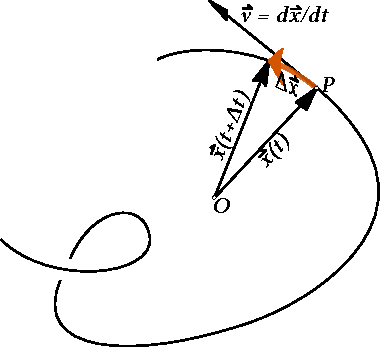
\includegraphics{005velocityistangent.pdf}
  \caption{The parametric curve $\vx(t)$ traces out a curve in space.  The vector
    $\vx(t)$ is the position vector of a point $P$ on this curve.  As we increase
    time from $t$ to $ t+\Delta t$, the point $P$ moves.  The displacement of the
    point $P$ is given by $\Delta\vx = \vx(t+\Delta t) - \vx(t)$.  The average
    velocity vector during
    this displacement is ``displacement/time'', i.e.\ $\Delta \vx/\Delta t$.\\
    \null\qquad If we let $\Delta t\to 0$, then the average velocity becomes the
    instantaneous velocity at time $t$: $\vv = \lim_{\Delta t\to0}\Delta\vx/\Delta t
    = \vv'(t)$.  This vector is tangential to the curve traced out by the vector
    function $\vx(t)$. }
  \label{fig:05velocity-is-deriv-of-position}
\end{figure}
\subsection{Velocity vector of a point moving in space} %{{{2
\label{sec:velocity-of-vector-motion}
let $\vx(t)$ be the position vector of some moving point $P$.  To define its velocity
we go back to the notion that ``velocity'' is always ``displacement divided by time.''

In this case we consider two instances in time, say, time $t$ and time $t+ \Delta t$.
Then the position vectors of the point $P$ at these two different times are $\vx(t)$
and $\vx(t+\Delta t)$.  The displacement of the point $P$ between these two times is
then
\[
  \Delta \vx = \vx(t+\Delta t) - \vx(t)
\]
(see Figure~\ref{fig:05velocity-is-deriv-of-position}.)  We say that the average
velocity over the time interval from $t$ to $t+\Delta t$ is ``the displacement
divided by $\Delta t$,'' i.e.
\[
  \vv_{\rm average} = \frac{\vx(t+\Delta t) - \vx(t)}{\Delta t}.
\]
Note that the average velocity is a vector.  If we write it out in components, we get
a much larger formula:
\[
  \vv_{\rm average} = \vek
  \dfrac{x(t+\Delta t) - x(t)}{\Delta t} \\[2ex]
  \dfrac{y(t+\Delta t) - y(t)}{\Delta t} \\[2ex]
  \dfrac{z(t+\Delta t) - z(t)}{\Delta t}
  \tor.
\]
One big advantage of using vector notation is that many formulas are much shorter when
written in terms of vectors.

To get the instantaneous velocity, we do the same thing as in one variable calculus:
we take the limit as $\Delta t\to0$ of the average velocity over the time interval
from $t$ to $t+\Delta t$.  Thus we get
\begin{equation}
  \vv(t) = \lim_{\Delta t\to0} \frac{\vx(t+\Delta t) - \vx(t)}{\Delta t} 
  \stackrel{\rm def}=
  \frac{d\vx}{dt}.
  \label{eq:velocity-of-vector-motion}
\end{equation}
In terms of components this derivative is 
\[
  \vx'(t)= \frac{d\vx}{dt} = \vek x'(t) \\ y'(t) \\ z'(t) \tor.
\]
Thus to compute the velocity (or derivative) corresponding to any given vector motion
$\vx(t)$ we can simply differentiate each separate component of $\vx(t)$.

\subsection{Acceleration} %{{{2
The \emph{acceleration vector} is
\[
\va(t) = \frac{d\vv}{dt} = \frac{d^2\vx} {dt^2} = \vek x''(t)\\ y''(t) \\ z''(t) \tor.
\]


\subsection{Example--motion on a straight line} %{{{2
Consider the motion given by
\begin{equation}
  \vx(t) = \va + t\vv
  \label{eq:straight-line-constant-velocity}
\end{equation}
where $\va $ and $\vv$ are given constant vectors.  To see what this
motion looks like let's plot a few vectors $\vx(t)$ for different
values of $t$?  At time $t=0$ we have $\vx(0) = \va$; at time $t=1$ we
have $\vx(1) = \va+\vv$, so in one time unit our point has moved by
the vector $\vv$; another time unit later, we have $\vx(2) =
\va+2\vv$, so that the point moved again by the vector $\vv$.
\begin{figure}[h]
  \centering
  \input ../figures/234/005linear-motion.pdf_tex
  \caption{\textbf{Vector form of linear motion: } the initial point
    has positions vector $\va$, }
  \label{fig:vector-form-linear-motion}
\end{figure}
After time $t$ has gone by, the position vector of the point is
$\vx(t) = \va+t\vv$, so that the point has moved by $t\vv$ since the
initial time $t=0$.  We say that $\vx(t)$ given by
\eqref{eq:straight-line-constant-velocity} describes motion with
constant velocity, whose velocity vector is $\vv$.

Here is another reason why we call $\vv$ the velocity vector.  In
general the average velocity of an object over some time interval
$t_0<t<t_1$ is the ratio between ``distance traveled'' and the time
that went by.  In the context of a 

As the point moves around in the plane or in space, it traces out a
curve.  The velocity vector $\vv(t) = \vx'(t)$ is always tangent to
the curve.

The \emph{length} of the curve traced out by $\vx(t), a\le t\le b$ is
given by
\[
s = \int_{t=a}^b \|\vx'(t)\|\; dt.
\]


\section{Arc length and the arc length derivative} %{{{1
Recall definition of arc length
\begin{equation}
  \label{eq:arclength-def}
  s = \int \|\vx'(t)\|\; dt.
\end{equation}
and arc length derivative:
\begin{equation}
  \frac{df}{ds} \isdef
  \lim_{\Delta t\to 0} 
  \frac{f(t+\Delta t) - f(t)}{s(t+\Delta t) - s(t)}
  \label{eq:arc-length-deriv-def}
\end{equation}
To compute use:
\begin{equation}
  \frac{df}{ds} = \frac{1}{\|\vx'(t)\|} \frac{df(t)}{dt}.
  \label{eq:arclenght-deriv}
\end{equation}
\section{Curvature} %{{{1
\begin{equation}
  \vT = \frac{d\vx}{ds} = \frac{\vx'(t)}{\|\vx'(t)\|}
  \label{eq:unit-tangent-def}
\end{equation}
\begin{equation}
  \frac{d\vT}{ds} = \kappa\; \vN 
  \label{eq:first-Serret-Frenet}
\end{equation}
\begin{equation}
  \frac{d\vN}{ds} = -\kappa\vT + \tau\; \vB 
  \label{eq:second-Serret-Frenet}
\end{equation}
where
\[
\vB= \vT\cp\vN.
\]
\begin{equation}
  \frac{d\vB}{ds} = -\tau\; \vN 
  \label{eq:third-Serret-Frenet}
\end{equation}

\section{Osculating plane} %{{{1

\section{Special cases: 2D} %{{{1
\begin{equation}
  \kappa = \frac{y''}{\bigl(1+(y')^2\bigr)^{3/2}}
  \label{eq:curvature-of-graph}
\end{equation}
\begin{equation}
  \kappa = \frac{d\theta}{ds}
  \label{eq:curvature-is-deriv-of-tangentangle}
\end{equation}
\section{Problems} %{{{1
\problemfont
\problem Suppose a point $P$ is rotating around a line $l$, keeping %{{{3
its distance to the line fixed at $r$, and moving in a plane
perpendicular to the line.  Suppose the point has angular velocity
$\omega$: this means that the angle swept out by the line from $P$ to
$l$ during a time interval of length $t$ is exactly $\omega t$.

In a previous math or physics class it was shown that the velocity of
the point $P$ is $\omega r$, where $r$ is the distance from $P$ to
$l$.

The \emph{angular velocity vector} is defined to be the vector
$\vvv\omega$ whose length is $\omega$, and which is parallel to the
line $l$.  There are two such vectors ($\pm \vvv\omega$).  By
definition $\vvv\omega$ points in the direction in which a corkscrew
would move if it were turning in the same direction as the point $P$.

\begin{figure}[h]
  \begin{center}
    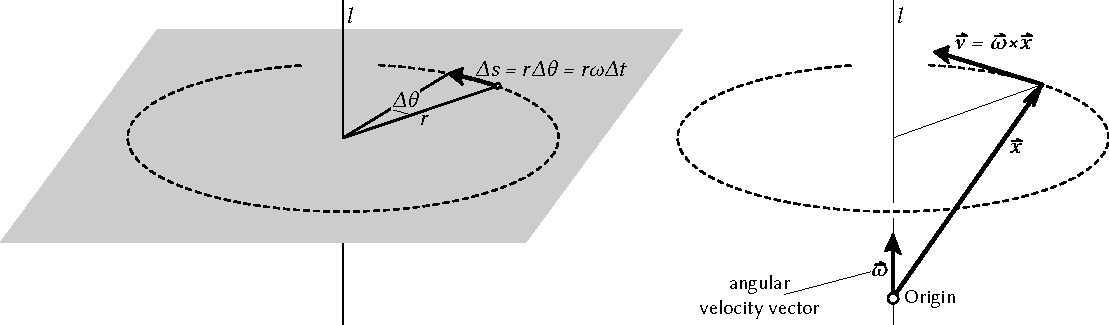
\includegraphics[width=0.9\textwidth]{005angularvelocity.pdf}
  \end{center}
\end{figure}


\subprob Assuming the line $l$ passes through the origin show that the
velocity vector of the point $P$ is $\vv = \vvv\omega \cp \vx$

\subprob Show that the acceleration vector is given by $\va =
\vvv\omega\cp(\vvv\omega\cp\vx)$.

\subprob If someone told you they had computed the acceleration vector
and found $\va =(\vvv\omega\cp\vvv\omega)\cp\vx$, could they be right?
Explain!  What if they told you they got $\va =
\vvv\omega\cp\vvv\omega\cp\vx$?

\subprob True or False (explain your answers):

(a) $\vv\perp \vx$?\qquad (b) $\va\perp \vv$? \qquad (c) $\va$ and
$\vx$ are parallel?

\subprob Include the acceleration vector $\va$ in the above drawing.

\problem Compute the curvature, torsion, tangent, normal and binormal %{{{3
for the following curves

\subprob The parabola: $\vx(t) = \tvek t^2 \\ t\ttor$.  At which point
on the curve is the curvature the largest?

\subprob Neil's parabola: $\tvek t^2\\ t^3\ttor$.  At which point on
the curve is the curvature the largest?

\subprob The helix: $\vx(\theta) =\vek\cos \theta \\ \sin \theta\\
a\theta\tor$ ($a>0$ is a constant).  At which point on the curve is
the curvature the largest?

\problem \subprob Compute the curvature at the point $(x, e^x)$ of the %{{{3
graph of $y=e^x$.
\answer $k(x) = \dfrac{e^x} %{{{3
{\bigl(1+e^{2x}\bigr)^{3/2}}$.
\endanswer

\subprob Which point on the graph of $y=e^x$ has the largest
curvature?
\answer $k'(x) = \dfrac{e^x} {\bigl(1+e^{2x}\bigr)^{5/2}} %{{{3
\bigl(1-2e^{2x}\bigr)$, so the maximal curvature (smallest radius of
curvature) occurs when $x=-\frac{1} {2}\ln{2}$.
\endanswer

\problem \subprob Compute the curvature at the point $(x, \ln x)$ of %{{{3
the graph of $y=\ln x$.

\subprob Which point on the graph of $y=\ln x$ has the largest
curvature?


\problem Show: a curve is plane if and only if its torsion vanishes %{{{3
($\tau = 0$).

\problem Express $\vx'\cp\vx''$ in terms of $\kappa, \tau, \vT, \vN, %{{{3
\vB$ and $\|\vx'\|$.

\problem Let $A(h)$ be the area of the triangle with vertices %{{{3
$\vx(t-h)$, $\vx(t)$ and $\vx(t+h)$.  Compute $\DS \lim_{h\to 0}
\frac{A(h)}{h^3}$.  Hint: use a Taylor expansion $\vx(t+h) = \vx(t) +
h\vx'(t) + \frac{h^2}{2}\vx''(t) + o(h^2)$.

\noproblemfont

\section{Line integrals} %{{{1
\begin{equation}
  \int_C f(\vx) ds
  \stackrel{\rm def}{=}
  \lim _{\Delta s_i\to0}
  \sum_{i=1}^N f(\vx_i) \Delta s_i
\end{equation}

Theorem:
\begin{equation}
  \int_C f(x, y) ds = \int_a^b f(\vx(t)) \nm{\vx'(t)}\; dt
\end{equation}


Definition:
\begin{equation}
  \int_C P(x, y, z)dx + Q(x, y, z)dy + R(x, y, z)dz
  =
  \int_a^b \bigl\{P(x, y, z)\frac{dx}{dt} +
  Q(x, y, z)\frac{dy}{dt} +
  R(x, y, z)\frac{dz}{dt}\bigr\} dt
  \label{eq:integral-of-one-form}
\end{equation}


%%% Local Variables: 
%%% mode: latex
%%% TeX-master: "free234"
%%% End: 
